
\documentclass[a4paper,11pt]{article}

\usepackage{amsmath,amssymb,amsfonts,amsthm}    % Typical maths resource packages
\usepackage{graphicx}                           % Packages to allow inclusion of graphics
\usepackage{hyperref}                           % For creating hyperlinks in cross references
\usepackage[bf]{caption2}
%\usepackage{natbib}                               % literature reference style
%\bibliographystyle{plainnat}
\usepackage[square,numbers]{natbib}
\bibliographystyle{plainnat}
\usepackage{enumitem}
% text formating
\usepackage{verbatim} 
% -------------------------------
% --- some layout definitions ---
% -------------------------------

% define topline
\usepackage[automark]{scrpage2}
\pagestyle{scrheadings}
\automark{section}
\clearscrheadings
\ohead{\headmark}


% define page size, margin size
\setlength{\headheight}{1.1\baselineskip}
\voffset=-2cm
\hoffset=-3cm
\textheight24cm
\textwidth15.5cm
\topmargin1cm
\oddsidemargin3cm
\evensidemargin3cm

% define line line spacing = 1.5
\renewcommand{\baselinestretch}{1.5}

% define second level for `itemizing'
\renewcommand{\labelitemii}{-}





% --------------------------------------
% --------------------------------------
% --------------------------------------
% --- the structure the tex document ---
% ---  (this our recommendation) -------
% frontmatter:
%   - titlepage (mandatory),
%   - acknowledgement,
%   - abstract,
%   - table of contents (mandatory),
%   - list of abbreviations (not mandatory),
%   - list of figures (not mandatory),
%   - list of tables  (not mandatory) .
%
% body of the thesis (the structure of the thesis body is not mandatory, but the list of literature is mandatory):
%   - introduction,
%   - methods,
%   - data,
%   - results,
%   - conclusion,
%   - literature (mandatory),
%   - appendix (figures, tables).
%
% last page:
%   - declaration of authorship (mandatory).
% --------------------------------------
% --------------------------------------
% --------------------------------------

\begin{document}

%% -------------------------------
%% --- frontmatter: Title page ---
%% -------------------------------
%
%\thispagestyle{empty}
%\begin{center}

    {\Large{\bf Fault-tolerant Syntax Error Validation for RDF Turtle  }} \vspace{0.5cm}


    {\normalsize Master's Thesis submitted\\\vspace{0.5cm}
    to}\\\vspace{0.5cm}
    {\normalsize{\bf Prof. Dr. Jens  Lehmann}} \\\vspace{0.5cm}
    {\normalsize Universit\"at  Bonn \\
    Computer Science Institute  \\} \vspace{1cm}


    {\normalsize by \\\vspace{0.5cm}
    {\bf Ahmad Hemid} \\
    ()} \vspace{1cm}


    {\normalsize in partial fulfillment of the requirements \\
    for the degree of \\
    {\bf Master of Science} \\
    Bonn, April 30, 2018}

\end{center}

%
%
%
%% ------------------------------------
%% --- frontmatter: Acknowledgement ---
%% ------------------------------------
%\newpage
%\pagestyle{plain}
%\pagenumbering{roman}   % define page number in roman style
%\setcounter{page}{1}    % start page numbering
%\section*{Acknowledgement}

I would like to thank

%
%
%
%% -----------------------------
%% --- frontmatter: Abstract ---
%% -----------------------------
%\newpage
%\section*{Abstract}

This is the template for a thesis at the Chair of Econometrics of
Humboldt--Universit\"at zu Berlin. A popular approach to write a
thesis or a paper is the IMRAD method (Introduction, Methods,
Results and Discussion). This approach is not mandatory! You can
find more information about formal requirements in the booklet
`Hinweise zur Gestaltung der \"au\ss eren Form von Diplomarbeiten'
which is available in the office of studies.\\

The abstract should not be longer than a paragraph of around 10 to
15 lines (or about 150 words). The abstract should contain a
concise description of the econometric/economic problem you
analyse and of your results. This allows the busy reader to obtain
quickly a clear idea of the thesis content.

%
%
%
%% -----------------------------
%% --- frontmatter: Contents ---
%% -----------------------------
%\newpage
%\tableofcontents
%\clearpage
%
%
%% ----------------------------------------------------
%% --- frontmatter: List of Figures (not mandatory) ---
%% ----------------------------------------------------
%\newpage
%\addcontentsline{toc}{section}{List of Abbreviations}
%\ohead[]{LIST OF ABBREVIATIONS}
%\section*{List of Abbreviations}

\begin{tabular}{rp{0.2cm}lp{1cm}rp{0.2cm}l}
    CPI     & &  Consumer Price Index   & & ETF     & &  Equity Traded Funds  \\
    ETH     & &  Eat the Horse          & & XLM     & &  Xetra Liquidity
\end{tabular}

%
%
%
%% ----------------------------------------------------
%% --- frontmatter: List of Figures (not mandatory) ---
%% ----------------------------------------------------
%\newpage
%\addcontentsline{toc}{section}{List of Figures}
%\ohead[]{\rightmark}
%\listoffigures
%
%
%
%% ---------------------------------------------------
%% --- frontmatter: List of Tables (not mandatory) ---
%% ---------------------------------------------------
%\newpage
%\addcontentsline{toc}{section}{List of Tables}
%\listoftables
%


% -------------------------------
% --- main body of the thesis ---
% -------------------------------
\newpage
\pagestyle{plain}
\setcounter{page}{1}    % start page numbering anew
\pagenumbering{arabic}  % page numbers in arabic style

\section{Introduction}

\begin{itemize}

    \item What is the subject of the study? Describe the
        economic/econometric problem.

    \item What is the purpose of the study (working hypothesis)?

    \item What do we already know about the subject (literature
        review)? Use citations: {\it \citet{Gallant:87} shows that...
        Alternative Forms of the Wald test are considered
        \citep{Breusch&Schmidt:88}.}

    \item What is the innovation of the study?

    \item Provide an overview of your results.


    \item Outline of the paper:\\
        {\it The paper is organized as follows. The next section describes the
        model under investigation. Section \ref{Sec:Data} describes the data set
        and Section \ref{Sec:Results} presents the results. Finally, Section
        \ref{Sec:Conc} concludes.}

    \item The introduction should not be longer than 4 pages.

\end{itemize}

\newpage
\section{Background} \label{Sec:Background}   
   
\newpage
\section{Literature Review} \label{Sec:Review}
In order to validate RDF code, either by pasting URL where it exists or by uploading a file, almost the available tools and applications that we could find, will only give the first occurred error. Moreover, semantic developers and engineers will struggle in debugging their codes and they need alternative tools that could be more helpful. To the best of our knowledge, there is no comparable prior work regarding fault-tolerant tool to validate syntactically RDF serialization formats expect one that works only for RDF/XML format, the following text sheds light on this tool. The new proposed tool should feature prominently in listing of all errors included in the code.

This section reviews the related research works have been done and presents the current state of the art of RDF syntax validating. Despite the long record of RDF syntax validation research with many of theoretical models or practical tools, we can hardly find a research that describes the challenge of detection multiple syntax errors inside RDF code. During our journey of checking the existing tools that provide such validation service, The W3C RDF validation tool \citep{W3C:Validation:Online} was firstly checked, it is available online for parsing and validating RDF/XML codes. It uses the ARP parser of Jena \citep{McBride:2002:JSW:613357.613755} as a backend. However, it fails in detection of multiple syntax errors, the first error in the order will be only released. K. Tolle developed a Validating RDF Parser (VRP) \citep{karsten:Thesis:2000} in his thesis, VRP is a Java-based build tool, and it validates RDF/XML code semantically and syntactically. Nevertheless, the validation service provided by VRP is limited to RDF/XML and does not support other RDF serialization formats, especially those formats which are structured in triples such as N3, NTriple, and Turtle. In this work, extension of syntax validation to other formats is planned. 

The journey to check the existing tools that validate RDF serialization formats other than RDF/XML is continued. As previously stated, Jena RDF toolkit \citep{McBride:2002:JSW:613357.613755} offers validation service based on ARP parser. It can be used as a command-line program (standalone) or as an API within another application. Despite its ability to validate numerous RDF serialization formats, including RDF/XML, again, the first error is only reported. Some of the tools validating RDF formats use the following core techniques as a significant part of their implementations:
\begin{itemize}[noitemsep] 
\item \textbf{ARP-parser-dependable approach :} both W3C RDF validation tool \citep{W3C:Validation:Online} and RDF Validator and Converter \citep{Mybluemix:Validation:Online} use ARP parser of Jena \citep{McBride:2002:JSW:613357.613755}. Moreover, the latter focuses more on triple-based serialization formats, validating them and converting from one format to another, where the former validates only RDF/XML format. 
\item \textbf{N3-parser-dependable approach :} N3 parser can also be used for syntax validation. In the online IDLab Turtle Validator \citep{IDLab:Validation:Online}, N3 parser powered by N3 NodeJS library is used. As well, same approach was used to build a turtle editor with syntax validation in \citep{petersenturtleeditor}. 
\item \textbf{Shape expressions approach :} in \citep{prud2014shape} a turtle parser was developed based on shape expressions. Shape expressions validates RDF through declaring of constraints on the RDF model, if the declared constraints are violated, then RDF is invalid. Furthermore, Shape expressions describes the RDF graph on regular expressions base. 
\end{itemize} 

When it comes to the application side, N3-parser-dependable approach can be fitted perfectly in the new tool, since it is built using Nodejs library. This can improve the performance of the tool, especially when it is validating a large RDF code. Moreover, the first two approaches are more expressive in explaining the syntax error and its location, where as, the tool used the third approach is less expressive.


In this research, our intention goes toward inventing a fancy tool that lists all syntax errors with an improved performance. The proposed tool can have a solution for the explained issue in either two ways: 
\begin{itemize}[noitemsep] 
\item \textbf{Patching the output errors of parsers :} while reviewing the source codes of others' tools, an error event by an error handler will be emitted to show the first occurred error. An idea of looping inside the RDF code and  fixing eachtime the first error can be suggested. Fixing the error can be by either deleting the triple made the error, removing or adding a punctuation, inserting a dummy IRI for an incorrect or missing one,  etc, then reprase the RDF code again and again till the end of the code .
\item \textbf{Parser Optimization :} this needs to review deeply the whole code of the parser and improve its method. The improvement should list all syntax errors that the parser can detect. Both parsers built with N3-parser-dependable approach or Shape expressions approach can be optimized to reach our goals while the optimization of the latter inherits more complexity. 
\end{itemize} 
 
To end this section, after describing the actual issue, reviewing the state of art of research works related to it, and finally presenting the possible solutions, we can say that both two solutions can solve the issue, but it seems to us that the second solution more efficient than the first, since this is the normal way how acually most of editors of programming languages work, to alert on-the-fly syntax errors to the programmer, even before compilation . 





%\begin{itemize}



% \item What is the subject of the study? Describe the
% economic/econometric problem.
%
% \item What is the purpose of the study (working hypothesis)?
%
% \item What do we already know about the subject (literature
% review)? Use citations: {\it \citet{Gallant:2018} shows that...
% Alternative Forms of the Wald test are considered
% \citep{Breusch&Schmidt:88}.}
%
% \item What is the innovation of the study?
%
% \item Provide an overview of your results.
%
%
% \item Outline of the paper:\\
% {\it The paper is organized as follows. The next section describes the
% model under investigation. Section \ref{Sec:Data} describes the data set
% and Section \ref{Sec:Results} presents the results. Finally, Section
% \ref{Sec:Conc} concludes.}
%
% \item The introduction should not be longer than 4 pages.

%\end{itemize}


\newpage
\section{Approach} \label{Sec:Approach} 
\subsection{Problem Description}
\subsection{Proposed Solution}
\subsubsection{Solution Architecture}

\newpage
\section{Implementation} \label{Sec:Implementation}   

\newpage
\section{Evaluation}\label{Sec:Evaluation}
\newpage
\section{Conclusions}\label{Sec:Conc}

\begin{itemize}

    \item Give a short summary of what has been done and what has been
    found.

    \item Expose results concisely.

    \item Draw conclusions about the problem studied. What are the
    implications of your findings?

    \item Point out some limitations of study (assist reader in judging validity
    of findings).

    \item Suggest issues for future research.

\end{itemize}







% literature
\newpage
\addcontentsline{toc}{section}{References}
\bibliography{literature}

% ----------------
% --- appendix ---
% ----------------
\appendix
\newpage
\let\cleardoublepage\clearpage
\begin{appendices}
\chapter{RDF-Doctor Grammar}
\label{ch:appendix}
% Applies only when you use it
\lstset{
    basicstyle=\color{black}\ttfamily,%
    breaklines=true,%                                      allow line breaks
    moredelim=*[s][\color{black}\ttfamily]{options}{\}},%  options in black (until trailing })
    commentstyle={\color{gray}\itshape},%                  gray italics for comments
    morecomment=[l]{//},%                                  define // comment
    emph={%
        STRING%                                            literal strings listed here
        },emphstyle={\color{blue}\ttfamily},%              and formatted in blue
    alsoletter={:,|,;},%
    morekeywords={:,|,;},%                                 define the special characters
    keywordstyle={\color{black}},%                         and format them in black
}

\begin{lstlisting}
// title of the grammar
grammar Turtle;
// functions in Java as a target programming language for RDF-Doctor parser
@parser::members { 
// Add member functions to check a Namespace declaration
public List<String> symbols = new ArrayList<String>();
boolean isExistNS(String in ) { 
	boolean foundNS = false ; 
		if(symbols.contains(in.split(":")[0]+':')) foundNS=true;
	return foundNS;
}
}
// the beginning of the grammar rules with 'start' root node
start
    : statement*  EOF
    ;
// 'statement' is a rule for either a triple or a prefix
statement
    : directive
    |  IRIREF IRIREF IRIREF  graphLabel '.'
// 'notifyErrorListeners' is a function to announce the existence of an error with its corresponding error message, same is applied for next rules
    {notifyErrorListeners("Turtle is not NQOUDS");}
    | triple '.'
    | triple {notifyErrorListeners("Missing '.' at the end of a triple");}
    | triple ',' {notifyErrorListeners("Bad end of a triple with ','");}
    | triple ';' {notifyErrorListeners("Bad end of a triple with ';'");}
    | triple ('.')+ ('.')+ {notifyErrorListeners("Too many DOT");}
    | errors		
    ;
// 'directive' is a rule for either a base or a prefix declaration
directive
    : sparqlPrefix
    | sparqlBase 
    | prefixID   
    | base
    | unkonwnDecl
    | sparqlPrefix '.' {notifyErrorListeners("Extraneous '.' at the end of SPARQL prefix directive");}
    | sparqlBase '.' {notifyErrorListeners("Extraneous '.' at the end of SPARQL base directive");}
    ;
// a rule to match certain incorrect syntax patterns
errors	
    : iri '=' iri '.' {notifyErrorListeners("'=' sign cannot be used in Turtle");}
 	| iri '<=' iri '.'  {notifyErrorListeners("'<=' symbol cannot be used in Turtle");}
    | iri '=>' iri '.'  {notifyErrorListeners("'=>' symbol cannot be used in Turtle");}
 	| (iri '.')+ (iri '.')+  triple '.' {notifyErrorListeners("N3 paths cannot be used in Turtle");}
    | (iri '.')+ (iri '.')+  triple  {notifyErrorListeners("N3 paths cannot be used in Turtle");}
    | iri '^'  triple '.' {notifyErrorListeners("N3 paths cannot be used in Turtle");}
    | '@forAll' iri '.' {notifyErrorListeners(" '@forAll' cannot be used in Turtle ");}
    | '@forSome' iri '.' {notifyErrorListeners(" '@forSome' cannot be used in Turtle ");}
    | ('a'|CHARS)* '@a' ('a'|CHARS)* '.' {notifyErrorListeners(" '@a' cannot be used in Turtle ");}
    ;
 graphLabel
 	: 	IRIREF | BLANK_NODE_LABEL
 	;
 unkonwnDecl 	
    : '@keywords' ('a'|CHARS)*  '.' {notifyErrorListeners("@keywords is unkown directive in Turtle");}
	;
// a rule for a prefix declaration to match  correct and incorrect forms
prefixID
    : '@prefix' CHARS '.' ':' IRIREF '.' {notifyErrorListeners("Prefix-label cannot end with '.' ");}
    | '@prefix' '.' CHARS ':' IRIREF '.' {notifyErrorListeners("Prefix-label cannot start with '.' ");}
    | '@prefix' ':' IRIREF '.' { symbols.add(":");} { System.out.println(":" + $IRIREF.text);} 
    | '@prefix' PNAME_NS  IRIREF '.' {symbols.add($PNAME_NS.text);}  { System.out.println($PNAME_NS.text + $IRIREF.text);} 
    | '@prefix' PNAME_NS IRIREF ('.')+ ('.')+ {notifyErrorListeners("Too many DOT ");}
    | PNAME_NS IRIREF '.' {notifyErrorListeners("Missing Prefix keyword, use '@prefix'");}
    | '@prefix'   IRIREF '.' {notifyErrorListeners("Missing Prefix-label in Prefix directive");}
    | '@prefix' CHARS*  IRIREF '.'  {notifyErrorListeners("Missing ':' in Prefix directive");}
    ;
// a rule for a base declaration to match  correct and incorrect forms
base
    : '@base' IRIREF '.'
    | '@base' IRIREF ('.')+ ('.')+ {notifyErrorListeners("Too many DOT ");}
    ;
sparqlBase
    : KW_BASE  IRIREF 
    | '@BASE'   IRIREF '.'  {notifyErrorListeners("incorrect syntax form of base directive");}
    ;
sparqlPrefix
    : KW_PREFIX CHARS '.' ':' IRIREF  {notifyErrorListeners("Prefix-label cannot end with '.' ");}
    | KW_PREFIX '.' CHARS ':' IRIREF  {notifyErrorListeners("Prefix-label cannot start with '.' ");}
    | KW_PREFIX PNAME_NS IRIREF
    | KW_PREFIX ':' IRIREF
    | PNAME_NS IRIREF {notifyErrorListeners("Missing Prefix keyword, use 'PREFIX'");}
    | KW_PREFIX  IRIREF  {notifyErrorListeners("Missing Prefix-label in Prefix directive");}
    ;
// declare keywords
KW_BASE 
    : B A S E 
    ;
KW_PREFIX 
    : P R E F I X 
    ;
// rules for a triple with correct and incorrect forms
triple
    : subject predicateObjectList
    | blankNodePropertyList predicateObjectList?
    | subject ':' object 
    | subject verb {notifyErrorListeners("Object of a triple is missing");}
    ;
predicateObjectList
    : verb objectList (';' verb objectList)*
    | verb objectList (';' verb objectList)* ('.')+ {notifyErrorListeners("Too many dots ");}
    | verb objectList (';' verb )* {notifyErrorListeners("Object of a triple is missing");}
    | verb  (';' verb objectList)* {notifyErrorListeners("Object of a triple is missing");}
    | verb objectList (';' verb objectList)* (';' verb )+ (';' verb objectList)* {notifyErrorListeners("Object of a triple is missing");}
    ;
objectList
    : object (',' object)*
    ;
// a rule for a predicate in a triple with correct and incorrect forms
verb
    :   'a' 
    | predicate
    | 'is' predicate 'of' {notifyErrorListeners("'is .. of' pattern is not used in Turtle");}
    | 'A' {notifyErrorListeners("'A' cannot be used as predicate, it should be replaced with 'a'");}
    | BooleanLiteral {notifyErrorListeners("Predicate cannot be a Boolean value");}
    | NumericLiteral  {notifyErrorListeners("Predicate cannot be a number");}
    | literal {notifyErrorListeners("Predicate cannot be a literal");}
    | BlankNode {notifyErrorListeners("Predicate cannot be a blank node");}
    ;
// a rule for a subject in a triple with correct and incorrect forms
subject
    : iri
    | BlankNode
    | BlankNode  '.' {notifyErrorListeners("Blank Node cannot be followed by '.'");}
    | 'a' {notifyErrorListeners("'a' cannot be used as a subject");}
    | BooleanLiteral {notifyErrorListeners("Subject cannot be a Boolean value");}
    | NumericLiteral  {notifyErrorListeners("Subject cannot be a number");}
    | rdfLiteral   {notifyErrorListeners("Subject cannot be a string");}
    | collection
    | '{' triple '.' '}' {notifyErrorListeners("{ } pattern cannot be used in Turtle");}
    | '{' triple '}' {notifyErrorListeners("{ } pattern cannot be used in Turtle");} 
    ;
predicate
    : iri
    ;
// a rule for an object in a triple with correct and incorrect forms
object
    : iri
    | BlankNode
    | collection
    | blankNodePropertyList
    | badBlankNodePropertyList  {notifyErrorListeners("incorrect form of a blank node list");}
    | literal
    | 'a' {notifyErrorListeners("'a' cannot be used as an object");}   
    ;
// a rule for literal replacing an object  with correct and incorrect forms
literal
    : rdfLiteral
    | NumericLiteral
    | BooleanLiteral
    | BadLiteral {notifyErrorListeners("incorrect form of a Literal");}
    ;
blankNodePropertyList
    : '[' predicateObjectList ']'
    ;
badBlankNodePropertyList   
	: '[' predicateObjectList '.' ']'
	;
collection
    : '(' object* ')'
    ;
NumericLiteral
    : INTEGER | DECIMAL | DOUBLE
    ;
rdfLiteral
    : BAD_STRING_LITERAL_LONG_QUOTE_WITH_OPEN_QUOTES  (LANGTAG | '^^' iri)?  {notifyErrorListeners("incorrect form of long literal with uncolsed qoutes");}
    | BAD_STRING_LITERAL_LONG_QUOTE_TOO_MANY (LANGTAG | '^^' iri)? {notifyErrorListeners("incorrect form of long literal with 4 qoutes");}
    | BAD_STRING_LITERAL_LONG_SINGLE_QUOTE_TOO_MANY (LANGTAG | '^^' iri)? {notifyErrorListeners("incorrect form of long literal with 4 qoutes");}
    | String  BAD_LANGTAG_AS_NUMBER  {notifyErrorListeners("Language tag cannot be a numeric value");}
    | String '^' iri {notifyErrorListeners("Missing '^' Character");}
    | String LANGTAG '^^' iri {notifyErrorListeners("incorrect form of a Literal");}
    | String '^^' iri LANGTAG {notifyErrorListeners("incorrect form of a Literal");}  
    | (BAD_STRING_LITERAL_LONG_SINGLE_QUOTE | BAD_STRING_LITERAL_LONG_QUOTE ) (LANGTAG | '^^' iri)?  {notifyErrorListeners("incorrect quotes of a literal");}
    | BAD_STRING_LITERAL_SINGLE_QUOTE (LANGTAG | '^^' iri)? {notifyErrorListeners("incorrect quotes of a literal");}
    | BAD_STRING_LITERAL_QUOTE (LANGTAG | '^^' iri)? {notifyErrorListeners("incorrect quotes of a literal");}
    | (BAD_STRING_LITERAL_QUOTE_WITH_BAD_UCHAR | BAD_STRING_LITERAL_SINGLE_QUOTE_WITH_BAD_UCHAR | BAD_STRING_LITERAL_LONG_SINGLE_QUOTE_WITH_BAD_UCHAR | BAD_STRING_LITERAL_LONG_QUOTE_WITH_BAD_UCHAR) {notifyErrorListeners("Bad Unicode Characters, Only HEX Characters are allowed");}
    | (BAD_STRING_LITERAL_QUOTE_WITH_BAD_ESCAPE | BAD_STRING_LITERAL_SINGLE_QUOTE_WITH_BAD_ESCAPE | BAD_STRING_LITERAL_LONG_SINGLE_QUOTE_WITH_BAD_ESCAPE | BAD_STRING_LITERAL_LONG_QUOTE_WITH_BAD_ESCAPE) {notifyErrorListeners("Bad Literal Escape");}
    |  String (LANGTAG | '^^' iri)?
    ;
// a rule for BooleanLiteral which can be either true or false
BooleanLiteral
    : 'true' | 'false'
    ;
// a rule for incorrect literal patterns
BadLiteral 
    : NumericLiteral ('.')+ CHARS 
    | NumericLiteral CHARS 
    | '+' '-' NumericLiteral
    ;
String
    : STRING_LITERAL_QUOTE | STRING_LITERAL_SINGLE_QUOTE | STRING_LITERAL_LONG_SINGLE_QUOTE | STRING_LITERAL_LONG_QUOTE
    ;
// a rule for IRI to match either incorrect or correct patterns
iri
    : ':' BAD_PN_LOCAL_STARTS_WITH_TILDE {notifyErrorListeners("Bad syntax of Prefixed IRI, the local prefix namespace cannot contain '~'");}
    |    PN_LOCAL_BAD_WITH_DASH {notifyErrorListeners("Bad syntax of Prefixed IRI, the local prefix namespace cannot start with dash");}
    | PrefixedName {if (!isExistNS($PrefixedName.text)){ notifyErrorListeners($PrefixedName.text.split(":")[0] +": prefix in " + $PrefixedName.text + " is undefined");}}
    | IRIREF 
    | PN_PREFIX? ':'  BAD_PN_LOCAL_STARTS_WITH_PERCENT {notifyErrorListeners("Bad syntax of Prefixed IRI, the local prefix namespace cannot contain '%'");}
    | BAD_PNAME_LN_STARTS_WITH_DOT  {notifyErrorListeners("incorrect form of Prefix-label, it cannot start with '.'");} 
    | BAD_PNAME_LN_ENDS_WITH_DOT  {notifyErrorListeners("incorrect form of Prefix-label, it cannot end with '.'");} 
    | BAD_IRIREF_WITH_SPACE {notifyErrorListeners("Bad syntax of IRI, IRI cannot contain space or newline");}
    | BAD_IRIREF_WITH_MULTIPLE_ANGLE_BRACKETS {notifyErrorListeners("Bad syntax of IRI, Too many angle brackets in IRI");}
    | BAD_IRIREF_WITH_PARENTHESES {notifyErrorListeners("Bad syntax of IRI, IRI cannot contain unexpected characters");}
    ;
BlankNode
    : BLANK_NODE_LABEL 
    | ANON
    ;
// a rule to skip spaces, tabs and empty lines
WS
    : ([\t\r\n\u000C] | ' ') + -> skip
    ;
// a rule to skip comments starting with '#'
COMMENT				  
	: '#' ~[\r\n]* -> skip;
// LEXER rules
CHARS
    : [a-zA-Z]+ [0-9]*
	;
PN_PREFIX
    : PN_CHARS_BASE ((PN_CHARS | '.')* PN_CHARS)?
    ;
IRIREF
    : '<' (~[\u0000-\u0020<>"{}|^`\\] | UCHAR)* '>' 
    ;
PNAME_NS
    : PN_PREFIX? ':'
    ;
PrefixedName
    :  PNAME_NS | PNAME_LN
    ;
PNAME_LN
    : PNAME_NS PN_LOCAL 
    ;
BAD_PNAME_LN_STARTS_WITH_DOT	  
	 : '.' PN_PREFIX ':' PN_LOCAL 
	 ;
BAD_PNAME_LN_ENDS_WITH_DOT	  
	 : PN_PREFIX  '.:' PN_LOCAL 
	 ;
BLANK_NODE_LABEL
    : '_:' (PN_CHARS_U | [0-9]) ((PN_CHARS | '.')* PN_CHARS)?
    ;
LANGTAG
    : '@' [a-zA-Z] + ('-' [a-zA-Z0-9] +)*
    ;
BAD_LANGTAG_AS_NUMBER
    : '@' [0-9]+
    ;
INTEGER
    : [+-]? [0-9]+
    ;
DECIMAL
    : [+-]? [0-9]* '.' [0-9] +
    ;
DOUBLE
    : [+-]? ([0-9] + '.' [0-9]* EXPONENT | '.' [0-9] + EXPONENT | [0-9] + EXPONENT)
    ;
EXPONENT
    : [eE] [+-]? [0-9] +
    ;
STRING_LITERAL_LONG_SINGLE_QUOTE
    : '\'\'\'' (~[\u0027\u005C\u000A\u000D] | ECHAR | UCHAR  | '\n' )*  ('\'' | '\'\'')?  (~[\u0027\u005C\u000A\u000D] | ECHAR | UCHAR)* '\'\'\''  
    ;
STRING_LITERAL_LONG_QUOTE
    : '"""'  ((~ ["\\] | ECHAR | UCHAR | '\'') ('"' | '""')? (';'| ',' |'.')* (~ ["\\] | ECHAR | UCHAR | '\''))* '"""'
    ;
STRING_LITERAL_QUOTE
    : '"' (~[\u0022\u005C\u000A\u000D] | ECHAR | UCHAR)* '"' 
    ;
STRING_LITERAL_SINGLE_QUOTE
    : '\'' (~ [\u0027\u005C\u000A\u000D] | ECHAR | UCHAR | '"')* '\''
    ;
// rules for IRI to match incorrect forms 
BAD_IRIREF_WITH_SPACE
 	:  '<' (PN_CHARS | '.' | ':' | '/' | '\\' | '#' | '@' | '%' | '&' | UCHAR)* '\n>'
	| '<' (PN_CHARS | '.' | ':' | '/' | '\\' | '#' | '@' | '%' | '&' | UCHAR)* '\u0020>'
	| '<' (PN_CHARS | '.' | ':' | '/' | '\\' | '#' | '@' | '%' | '&' | UCHAR)* ANON_WS+ (PN_CHARS |'.' | ':' | '/' | '\\' | '#' | '@' | '%' | '&' | UCHAR)*'>'
	;
BAD_IRIREF_WITH_MULTIPLE_ANGLE_BRACKETS
	:'<' (PN_CHARS | '.' | ':' | '/' | '\\' | '#' | '@' | '%' | '&' | UCHAR)* '\u003C>'
	| '<' (PN_CHARS | '.' | ':' | '/' | '\\' | '#' | '@' | '%' | '&' | UCHAR)* '\u003E>'
	;
BAD_IRIREF_WITH_PARENTHESES 
    : '<' (PN_CHARS | '.' | ':' | '/' | '{'| '}' | '\\' | '#' | '@' | '%' | '&' | UCHAR)* '>'
	;
// rules for incorrect literals
BAD_STRING_LITERAL_SINGLE_QUOTE   
    : '\'\'\'' (~[\u0027\u005C\u000A\u000D] | ECHAR | UCHAR)* '\'' 
	| '\'' (~[\u0027\u005C\u000A\u000D] | ECHAR | UCHAR)* '\'\'\'' 
	;
BAD_STRING_LITERAL_QUOTE      
	: '"""' (~[\u0022\u005C\u000A\u000D] | ECHAR | UCHAR)* '"' 
	| '"' (~[\u0022\u005C\u000A\u000D] | ECHAR | UCHAR)* '"""' 
	| '"' (~[\u0022\u005C\u000A\u000D] | ECHAR | UCHAR)* '\'' 
	| '\'' (~[\u0022\u005C\u000A\u000D] | ECHAR | UCHAR)* '"' 	
	| '"''\'' (~[\u0022\u005C\u000A\u000D] | ECHAR | UCHAR)* '""' 			
	;  	  
BAD_STRING_LITERAL_LONG_SINGLE_QUOTE
	: '\'\'\'' (('\'' | '\'\'')? ([^'\\] | ECHAR | UCHAR | '"'))* '"""'
	;
BAD_STRING_LITERAL_LONG_QUOTE
	: '"""' (('"' | '""')? (~ ["\\] | ECHAR | UCHAR | '\''))* '\'\'\''
	|  '"""' (('"' | '""')? (~ ["\\] | ECHAR | UCHAR | '\''))* '"' '\''
	|  '"' '\'' (~ ["\\] | ECHAR | UCHAR | '\'')* '""'
	;
BAD_STRING_LITERAL_LONG_QUOTE_TOO_MANY
	: '"""'  (~ ["\\] | ECHAR | UCHAR )* '""""'
	| '""""' (('"' | '""')? (~ ["\\] | ECHAR | UCHAR ))* '"""' 
	;	
BAD_STRING_LITERAL_LONG_SINGLE_QUOTE_TOO_MANY
	: '\'\'\'' (~[\u0027\u005C\u000A\u000D] | ECHAR | UCHAR)*  '\'\'\'\''
	| '\'\'\'\''(~[\u0027\u005C\u000A\u000D] | ECHAR | UCHAR)*  '\'\'\''
	;
BAD_STRING_LITERAL_QUOTE_WITH_BAD_UCHAR
    : '"' (~[\u0022\u005C\u000A\u000D] | ECHAR | UCHAR)* BAD_UCHAR (~[\u0022\u005C\u000A\u000D] | ECHAR | UCHAR)* '"' 
    ;
BAD_STRING_LITERAL_SINGLE_QUOTE_WITH_BAD_UCHAR
    : '\'' (~ [\u0027\u005C\u000A\u000D] | ECHAR | UCHAR | '"')*  BAD_UCHAR (~ [\u0027\u005C\u000A\u000D] | ECHAR | UCHAR | '"')*  '\''
    ;
BAD_STRING_LITERAL_LONG_SINGLE_QUOTE_WITH_BAD_UCHAR
    : '\'\'\'' (~[\u0027\u005C\u000A\u000D] | ECHAR | UCHAR  | '\n' )*  ('\'' | '\'\'')?  (~[\u0027\u005C\u000A\u000D] | ECHAR | UCHAR)* BAD_UCHAR   (~[\u0027\u005C\u000A\u000D] | ECHAR | UCHAR  | '\n' )*  ('\'' | '\'\'')?  (~[\u0027\u005C\u000A\u000D] | ECHAR | UCHAR)*'\'\'\''  
    ;
BAD_STRING_LITERAL_LONG_QUOTE_WITH_BAD_UCHAR
    : '"""'  (~[\u0022\u005C\u000A\u000D] | ECHAR | UCHAR)*   BAD_UCHAR (~[\u0022\u005C\u000A\u000D] | ECHAR | UCHAR)*   '"""'
    ;
BAD_STRING_LITERAL_LONG_QUOTE_WITH_OPEN_QUOTES
    : '"""'  (~ ["\\] | ECHAR | UCHAR )* '\n' '\n'
    ;
BAD_STRING_LITERAL_QUOTE_WITH_BAD_ESCAPE
    : '"' (~[\u0022\u005C\u000A\u000D] | ECHAR | UCHAR)* ILLEGAL_ESCAPE (~[\u0022\u005C\u000A\u000D] | ECHAR | UCHAR)* '"' 
    ;
BAD_STRING_LITERAL_SINGLE_QUOTE_WITH_BAD_ESCAPE
    : '\'' (~ [\u0027\u005C\u000A\u000D] | ECHAR | UCHAR | '"')*  ILLEGAL_ESCAPE (~ [\u0027\u005C\u000A\u000D] | ECHAR | UCHAR | '"')*  '\''
    ;
BAD_STRING_LITERAL_LONG_SINGLE_QUOTE_WITH_BAD_ESCAPE
    : '\'\'\'' (~[\u0027\u005C\u000A\u000D] | ECHAR | UCHAR  | '\n' )*  ('\'' | '\'\'')?  (~[\u0027\u005C\u000A\u000D] | ECHAR | UCHAR)* ILLEGAL_ESCAPE   (~[\u0027\u005C\u000A\u000D] | ECHAR | UCHAR  | '\n' )*  ('\'' | '\'\'')?  (~[\u0027\u005C\u000A\u000D] | ECHAR | UCHAR)*'\'\'\''  
    ;
BAD_STRING_LITERAL_LONG_QUOTE_WITH_BAD_ESCAPE
    : '"""'  (~[\u0022\u005C\u000A\u000D] | ECHAR | UCHAR)*   ILLEGAL_ESCAPE (~[\u0022\u005C\u000A\u000D] | ECHAR | UCHAR)*   '"""'
    ;
// a rule for Unicode characters
fragment UCHAR
    : '\\u' HEX HEX HEX HEX | '\\U' HEX HEX HEX HEX HEX HEX HEX HEX
    ;
BAD_UCHAR
	: '\\u' HEX* NONHEX+ | '\\U' HEX* NONHEX+ 
	;
ECHAR
    : '\\' [tbnrf"'\\]
    ;
ANON_WS
    : ' ' | '\t' | '\r' | '\n'
    ;
ANON
    : '[' ANON_WS* ']'
    ;
PN_CHARS_BASE
    : [A-Z] | [a-z] | [\u00C0-\u00D6] | [\u00D8-\u00F6] | [\u00F8-\u02FF] | [\u0370-\u037D]
	| [\u037F-\u1FFF] | [\u200C-\u200D] | [\u2070-\u218F] | [\u2C00-\u2FEF] | [\u3001-\uD7FF]
	| [\uF900-\uFDCF] | [\uFDF0-\uFFFD]				   		   
    ;
PN_CHARS_U
    : PN_CHARS_BASE | '_'
    ;
PN_CHARS
    : PN_CHARS_U | '-' | [0-9] | '\u00B7' | [\u0300-\u036F] | [\u203F-\u2040]
    ;
PN_LOCAL
    : (PN_CHARS_U | ':' | [0-9] | PLX) ((PN_CHARS | '.' | ':' | PLX)* (PN_CHARS | ':' | PLX))?
    ;
// rules for incorrect fragments within Prefixed-Names
BAD_PN_LOCAL_STARTS_WITH_PERCENT
    :   '%' (PN_CHARS_U | ':' | [0-9]) ((PN_CHARS | '.' | ':' )* (PN_CHARS | ':' ))?
    ;
BAD_PN_LOCAL_CONTAINS_PERCENT
    : CHARS* '%' [0-9]
    ;
BAD_PN_LOCAL_STARTS_WITH_TILDE
    : [a-zA-Z] ('\u007E'|'\u02DC'|'\u0303'|'\u2053'|'\u223C'| '\uFF5E' ) [a-zA-Z]
    ;
PN_LOCAL_BAD_WITH_DASH
    : ':' '\u002D' [a-z]+
    ;
PLX
    : PERCENT | PN_LOCAL_ESC
    ;
PERCENT
    : '%' HEX HEX
    ;
HEX
    : [0-9] | [A-F] | [a-f]
    ;
NONHEX
	: [g-zG-Z]
	;
PN_LOCAL_ESC
    : '\\' ('_' | '~' | '.' | '-' | '!' | '$' | '&' | '\'' | '(' | ')' | '*' | '+' | ',' | ';' | '=' | '/' | '?' | '#' | '@' | '%')
    ;
ILLEGAL_ESCAPE
	: ('\\' ~[ubtnfr"'\\] ) [a-zA-Z]+ 
	;
// rules for the alphabet capital and small-letters
fragment A
    :('a'|'A')
    ;
fragment B
    :('b'|'B')
    ;
fragment C
    :('c'|'C')
    ;
fragment D
    :('d'|'D')
    ;
fragment E
    :('e'|'E')
    ;
fragment F
    :('f'|'F')
    ;
fragment G
    :('g'|'G')
    ;
fragment H
    :('h'|'H')
    ;
fragment I
    :('i'|'I')
    ;
fragment J
    :('j'|'J')
    ;
fragment K
    :('k'|'K')
    ;
fragment L
    :('l'|'L')
    ;
fragment M
    :('m'|'M')
    ;
fragment N
    :('n'|'N')
    ;
fragment O
    :('o'|'O')
    ;
fragment P
    :('p'|'P')
    ;
fragment Q
    :('q'|'Q')
    ;
fragment R
    :('r'|'R')
    ;
fragment S
    :('s'|'S')
    ;
fragment T
    :('t'|'T')
    ;
fragment U
    :('u'|'U')
    ;
fragment V
    :('v'|'V')
    ;
fragment W
    :('w'|'W')
    ;
fragment X
    :('x'|'X')
    ;
fragment Y
    :('y'|'Y')
    ;
fragment Z
    :('z'|'Z')
    ;	
\end{lstlisting}

\chapter{RDF Syntax Errors Categories}
\label{ch:synErrCategories}
\vspace{-5mm}
 \begin{table}[H]
 	\caption{\textbf{Categories of syntax errors of N-Triple and Turtle serializations.} These categories are extracted from files of Turtle Test Suite \cite{TurtleTests:Online}, including   incorrect syntactic forms.}
 \label{tab:syntaxErrorCate}
 	\centering
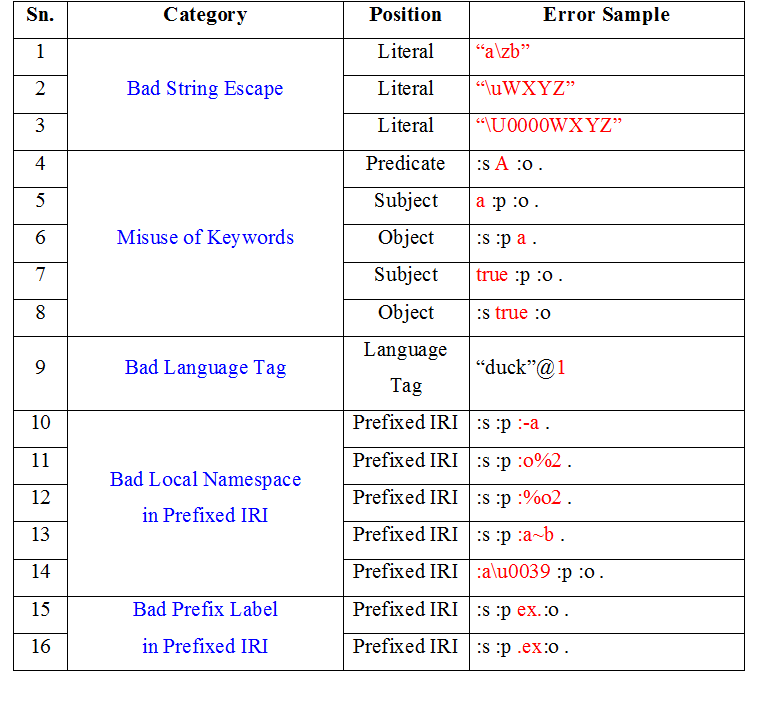
\includegraphics[width=5.5in]{images/bigTablePage1.png}
\end{table}

 \begin{figure}[H]
 	\centering
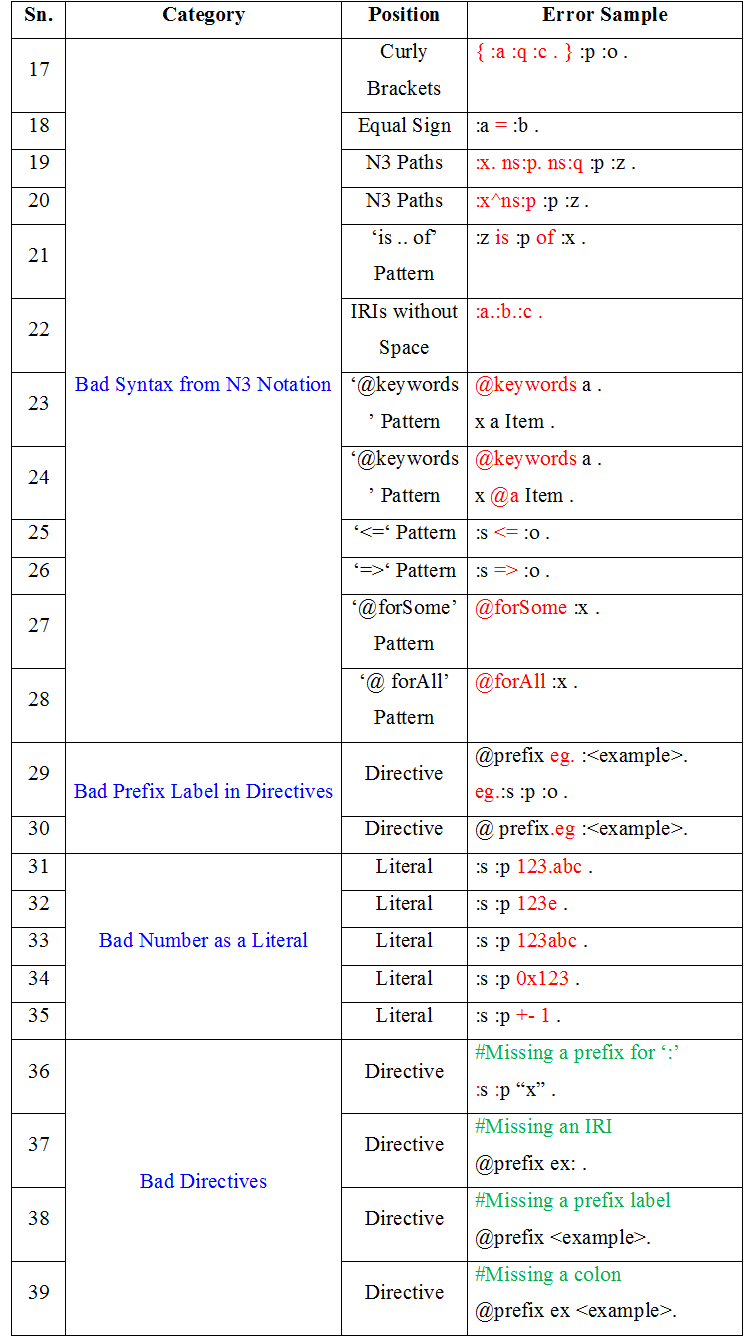
\includegraphics[width=5.5in]{images/bigTablePage3.png}
\end{figure}
 \begin{figure}[H]
 	\centering
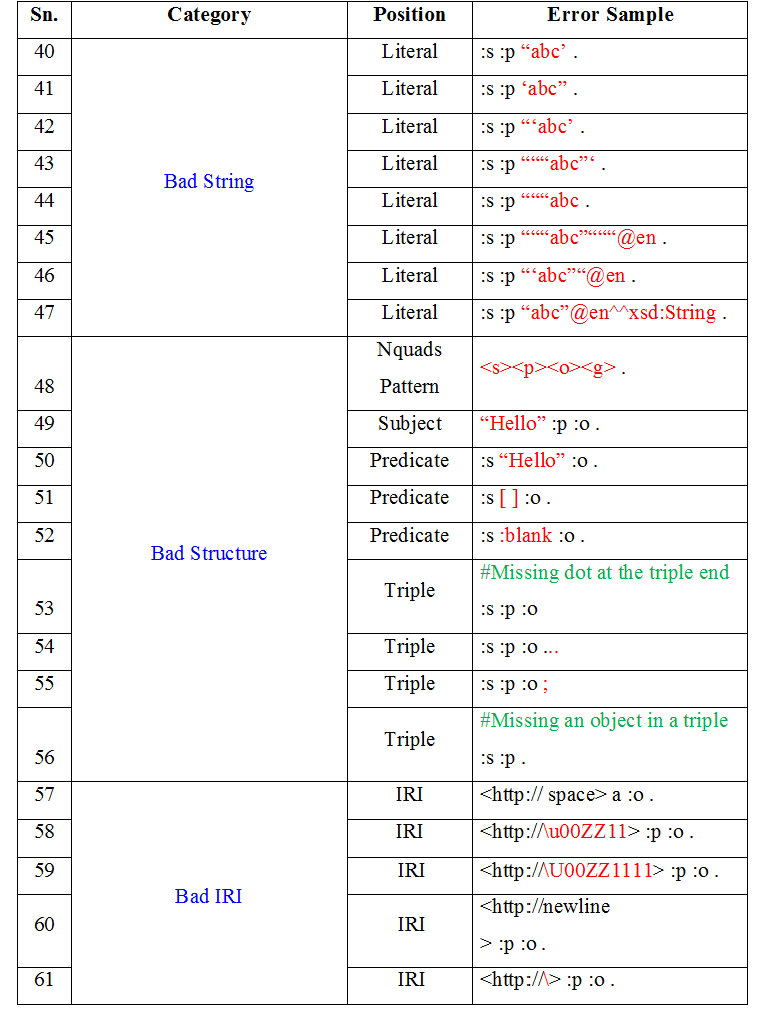
\includegraphics[width=5.5in]{images/bigTablePage7.png}
\end{figure}
%\includepdf[pages=2-3,pagecommand={},width=\textwidth,noautoscale=true,offset=80 30]{images/bigTable.pdf}
\end{appendices}


%% figures (not mandatory)
%\newpage
%\section{Figures}

\begin{figure}[ht]
    \begin{center}
        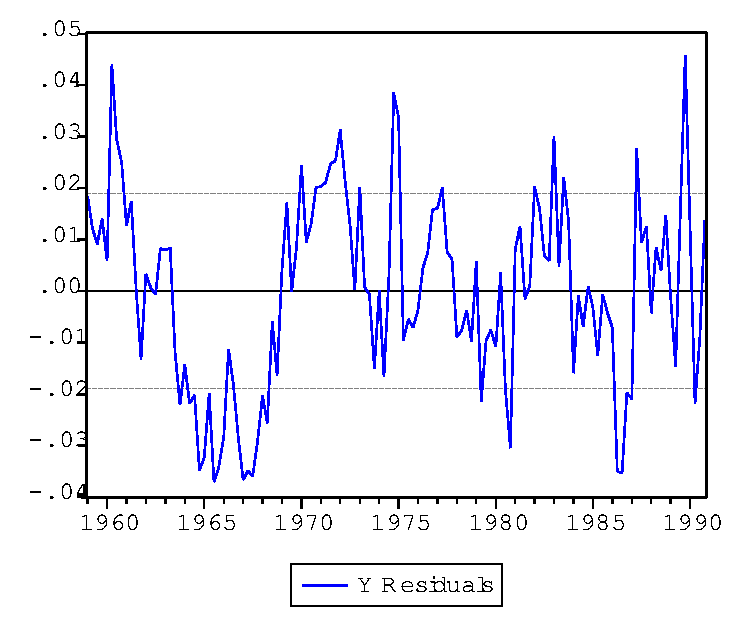
\includegraphics[scale=0.5,angle=0]{graph}
        \caption{Estimated residuals (2) from model XXX. ...}
        \label{Fig:Resids2}
    \end{center}
\end{figure}

%
%% tables (not mandatory)
%\newpage
%\section{Tables}

\begin{table}[ht]
    \begin{center}
        {\footnotesize
        \begin{tabular}{l|cccccccccc}
        \hline \hline
                        & 3m    & 6m    & 1yr   & 2yr   & 3yr   & 5yr   & 7yr   & 10yr  & 12yr  & 15yr   \\
            \hline
                Mean   & 3.138 & 3.191 & 3.307 & 3.544 & 3.756 & 4.093 & 4.354 & 4.621 & 4.741 & 4.878  \\
                Median & 3.013 & 3.109 & 3.228 & 3.490 & 3.680 & 3.906 & 4.117 & 4.420 & 4.575 & 4.759  \\
                Min    & 1.984 & 1.950 & 1.956 & 2.010 & 2.240 & 2.615 & 2.850 & 3.120 & 3.250 & 3.395  \\
                Max    & 5.211 & 5.274 & 5.415 & 5.583 & 5.698 & 5.805 & 5.900 & 6.031 & 6.150 & 6.295  \\
                StD    & 0.915 & 0.919 & 0.935 & 0.910 & 0.876 & 0.825 & 0.803 & 0.776 & 0.768 & 0.762  \\
            \hline \hline
        \end{tabular}}
    \end{center}
    \caption{Detailed descriptive statistics of location and dispersion for
    2100 observed swap rates for the period from
    February 15, 1999 to March 2, 2007. Swap rates measured as 3.12 (instead of 0.0312).}
    \label{Tab:DescripStatsRawDataDetail}
\end{table}




% --------------------------------------------
% --- last page: Declaration of Authorship ---
% --------------------------------------------
%
%\newpage
%\thispagestyle{empty}
%%{\Large{\bf Declaration of Authorship}}\vspace{0.5cm}

\section*{Declaration of Authorship}

I hereby confirm that I have authored this Bachelor's/Master's
thesis independently and without use of others than the indicated
sources. All passages which are literally or in general matter
taken out of publications or other sources are marked as such.
\vspace{1cm}

Bonn, April 30, 2018 \vspace{0.5cm}

Ahmad Hemid



\end{document}
